\documentclass[tikz,border=3mm,convert={density=600,outfile=\jobname.png}]{standalone}
%\documentclass[tikz,border=3mm]{standalone}
\usetikzlibrary{positioning}
\begin{document}
	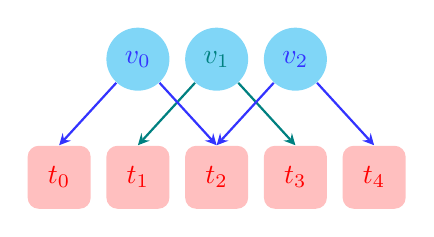
\begin{tikzpicture}
		[node distance=1cm,on grid,>=stealth,bend angle=45,auto,
		every valuenode/.style= {circle,minimum size=6mm,fill=cyan!50},
		every timenode/.style= {minimum size=8mm,fill=pink}]
		
		\node[fill=cyan!50, circle, minimum size=8mm] (v1) at (0,0) {\textcolor{teal}{$v_1$}};
		\node[fill=cyan!50, circle, minimum size=8mm] (v0) [left=of v1] {\textcolor{blue!80}{$v_0$}};
		\node[fill=cyan!50, circle, minimum size=8mm] (v2) [right=of v1] {\textcolor{blue!80}{$v_2$}};
		\node[fill=pink, rounded corners, minimum size=8mm,node distance=1.5cm] (t2) [below=of v1] {\textcolor{red}{$t_2$}} ;
		\node[fill=pink, rounded corners, minimum size=8mm] (t3) [right=of t2] {\textcolor{red}{$t_3$}};
		\node[fill=pink, rounded corners, minimum size=8mm] (t4) [right=of t3] {\textcolor{red}{$t_4$}};
		\node[fill=pink, rounded corners, minimum size=8mm] (t1) [left=of t2] {\textcolor{red}{$t_1$}};
		\node[fill=pink, rounded corners, minimum size=8mm] (t0) [left=of t1] {\textcolor{red}{$t_0$}};
		
		\draw[->, teal, thick] (v1) edge (t1.north)
		(v1) edge (t3.north);
		\draw[->, blue!80, thick]
		(v0) edge (t0.north)
		(v0) edge (t2.north)
		(v2) edge (t2.north)
		(v2) edge (t4.north);
		
	\end{tikzpicture}
\end{document}